%---------------------------------------------------------------------------------------------%
% Chapter: Koordinatentransformation
%---------------------------------------------------------------------------------------------%
Für die kinematische Modellierung von Hexapoden ist die korrekte Beschreibung ihrer Transformationsgleichungen von elementarer Bedeutung. Folglich sollen in diesem Abschnitt die Grundlagen der Koordinatentransformation in Ebene und Raum wiederholt werden. \\

%Mit den erarbeiteten mathematischen Grundoperationen soll im Anschluss ein Gleichungssystem zur Beschreibung der \glqq 6D-Transformation \grqq einer allgemeinen Hexapod-Kinematik aufgestellt werden.\\
%Die mobile Plattform einer Hexapod-Kinematik lässt sich in sechs Freiheitsgraden bewegen, wobei drei Translationen und drei Rotationen um jede der drei Raumachsen möglich sind. Die mathematische Beschreibung dieser kombinierten Bewegungen erfolgt im Allgemeinen über entsprechende Transformationsmatrizen die eine \glqq 6D-Transformation \grqq in nur einer Matrixoperation ermöglichen. Für die Aufstellung solcher Transformationsgleichungen bedarf es der Festlegung einer Konvention hinsichtlich der Transformationsfolge die sich je nach Anforderung an das kinematische System bzw. die Anwendung unterscheiden kann und damit die spezielle Form der Transformationsmatrix festlegt. Die Transformationsfolge definiert, in welcher Folge die rotatorischen Operationen gereiht sind und ob die Translationen vor oder nach den rotatorischen Transformationen einfließen. Häufige Festlegungen sind die \glqq Euler-Winkel-Konvention \grqq und die \glqq Roll-Nick-Gier-Konvention \grqq. \\

Unter einer Koordinatentransformation wird im Allgemeinen die Übersetzung von einem Koordinatensystem $K = \{O;\bvec{e_{i}}\}$ auf ein gleichartiges System $K^\prime = \{O^\prime;\bvec{e_{i}}^\prime\}$, $i=1,2,\ldots,n$ verstanden. Man unterscheidet zwei grundsätzliche Fälle:

\subsubsection{Fall A - Feststehendes System und bewegtes Objekt} 
Übergang von einer Objektkonfiguration $P$ in eine neue Konfiguration $P^\prime$ wobei das Koordinatensystem $K$ unverändert bleibt. Beispiel: {\color{red}Überwachung vom Flugverkehr mittels Radar, wobei der Kontrolltower das ortsfeste System $K$ stellt und die sich im Luftraum befindlichen Flugzeuge $P_{i}$ relativ zu $K$in eine neue Konfiguration $P_{i}^\prime$ bewegen.}
\subsubsection{Fall B - Bewegtes System und feststehendes Objekt}
Übergang vom System $K$ in ein gleichartiges System $K^\prime$ wobei die Objekte $P_{i}$ nicht transformiert werden. Beispiel: Bearbeitung eines eingespannten, also ortsfesten Werkstücks in einer Werkzeugmaschine. Das Werkzeugkoordinatensystem $K^\prime$ wird hierbei gemäß des CNC-Programms relativ zum Maschinenkoordinatensystem $K$ bewegt. 
\footcite[Vgl.][1-2]{Neugebauer2006}
\footcite[Vgl.][95]{Keferstein2018}
\footcite[Vgl.][8-20]{Wloka1994}
\footcite[Vgl.][38\psqq]{Bartsch2014}
\footcite[Vgl.][33]{Pfeifer2010}
\footcite[Vgl.][12]{Schuth2017}
%---------------------------------------------------------------------------------------------%
% Subsection: Koordinatentransformation in der Ebene
%---------------------------------------------------------------------------------------------%
\newpage
\subsection{Translation in der Ebene}
\label{subsec:translation_2d}
%---------------------------------------------------------------------------------------------%
% Fall A - Verschiebung des Objekts
%---------------------------------------------------------------------------------------------%
\subsubsection{Fall A - Verschiebung des Objekts}
Betrachtet werde ein Punkt $P$ in der $xy$-Ebene, dessen Position durch den Ortsvektor $\bvec{x}$ bestimmt sei, siehe \cref{fig:translation_2d_a}. Mit dem in \cref{eq:translation_2d_1} eingeführten Translationsvektor $\bvec{t}$ erfolgt eine Verschiebung von $P$ nach $P^\prime$. Der Übergang von $\bvec{x}$ in den neuen Ortsvektor $\bvec{x}^\prime$ wird durch die Transformationsgleichung \bref{eq:translation_2d_2} beschrieben.
%---------------------------------------------------------------------------------------------%
\begin{equation}
    \bvec{t} = t_{x}\bvec{{e_{x}}}+t_{y}\bvec{e_{y}} \label{eq:translation_2d_1}
\end{equation}
\begin{equation}
    \bvec{x}^\prime = \bvec{x}+\bvec{t} 
    \quad\Longleftrightarrow\quad
    \begin{cases}
        x^\prime=x+t_{x}\\
        y^\prime=y+t_{y}
    \end{cases}
    \label{eq:translation_2d_2}\\
\end{equation}
%---------------------------------------------------------------------------------------------%
% Fall B - Verschiebung des Ursprungs
%---------------------------------------------------------------------------------------------%
\subsubsection{Fall B - Verschiebung des Ursprungs}
\cref{fig:translation_2d_b} zeigt die Verschiebung des Ursprungs $O$ nach $O^\prime$ durch den in \cref{eq:translation_2d_1} eingeführten Translationsvektor $\bvec{t}$. Die Position von $P$ ändert sich nicht, stattdessen wird das System $K = \{O;\bvec{x},\bvec{y}\}$ in das System $K^\prime = \{O^\prime;\bvec{x}^\prime\,\bvec{y}^\prime\}$ übergeführt. Durch die Änderung des Bezugssystems erfolgt eine Transformation von $\bvec{x}$ nach $\bvec{x}^\prime$ gemäß \cref{eq:translation_2d_3}.
%---------------------------------------------------------------------------------------------%
\begin{equation}
    \bvec{x}^\prime = \bvec{x}-\bvec{t} 
    \quad\Longleftrightarrow\quad
    \begin{cases}
        x^\prime=x-t_{x}\\
        y^\prime=y-t_{y}
    \end{cases}
    \label{eq:translation_2d_3}
\end{equation}
Der Vorzeichenwechsel von \cref{eq:translation_2d_2} auf \cref{eq:translation_2d_3} macht deutlich, dass die Transformation von \textbf{Fall A} der \glqq inversen Transformation\grqq\ von \textbf{Fall B} entspricht, und umgekehrt. Die Wahl des Transformationsfalls entscheidet somit über die Transformationsrichtung. Dieses Merkmal ist charakteristisch für alle in weiterer Folge betrachteten Transformationsarten.
%---------------------------------------------------------------------------------------------%
% TikZ: Translation in der Ebene
%---------------------------------------------------------------------------------------------%
\begin{figure}[H]
    \centering
    \begin{subfigure}[b]{0.45\textwidth}
        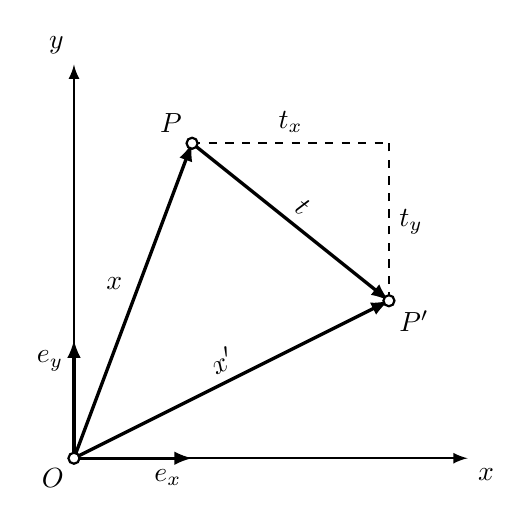
\begin{tikzpicture}
    %\sansmath
    %----------------------------------------------------------------------------------------%
    % Koordinaten
    %----------------------------------------------------------------------------------------%
    \coordinate (O) at (0,0);
    \coordinate (P1) at (1.5,4);
    \coordinate (P2) at (4,2);
    %----------------------------------------------------------------------------------------%
    % Koordinatenachsen
    %----------------------------------------------------------------------------------------%
    \begin{scope}[thick,->,>=latex]
    \draw (O) -- +(5,0) node[anchor=north west] {$x$};
    \draw (O) -- +(0,5) node[anchor=south east] {$y$};
    \end{scope}
    %----------------------------------------------------------------------------------------%
    % Einheitsvektoren
    %----------------------------------------------------------------------------------------%
    \begin{scope}[very thick,->,>=latex,scale = 1.5]
    \draw (O) -- +(1,0) node[anchor=north east] {$\boldsymbol{e_{x}}$};
    \draw (O) -- +(0,1) node[anchor=north east] {$\boldsymbol{e_{y}}$};
    \end{scope}
    %----------------------------------------------------------------------------------------%
    % Vektoren
    %----------------------------------------------------------------------------------------%
    \begin{scope}[very thick,->,>=latex]
    \draw (O) -- (P1) node [midway, anchor = south east] {$\boldsymbol{x}$};
    \draw (O) -- (P2) node [midway, sloped, above] {$\boldsymbol{x}^\prime$};
    \draw (P1) -- (P2) node [midway, sloped, above] {$\boldsymbol{t}$};
    \end{scope}
    %----------------------------------------------------------------------------------------%
    % Komponenten
    %----------------------------------------------------------------------------------------%
    \begin{scope}[thick, dashed]
    \draw (P1) -- (P2|-P1) node [midway, anchor = south] {$t_{x}$};
    \draw (P2) -- (P1-|P2) node [midway, anchor = west] {$t_{y}$};
    \end{scope}
    %----------------------------------------------------------------------------------------%
    % Punkte
    %----------------------------------------------------------------------------------------%
    \begin{scope}[thick,draw=black,fill=white]
    \filldraw (O) circle (2pt) node[anchor=north east] {$O$};
    \filldraw (P1) circle (2pt) node[anchor=south east] {$P$};
    \filldraw (P2) circle (2pt) node[anchor=north west] {$P^\prime$};
    \end{scope}
\end{tikzpicture}
        \caption{Verschiebung des Objekts}\label{fig:translation_2d_a}
    \end{subfigure}
    \begin{subfigure}[b]{0.45\textwidth}
        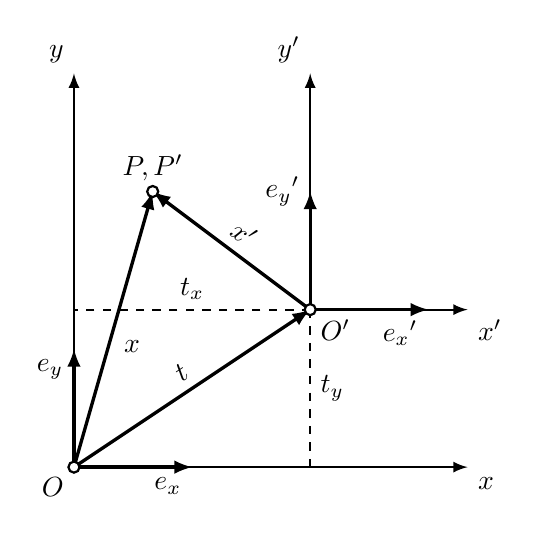
\begin{tikzpicture}
    %\sansmath
    %----------------------------------------------------------------------------------------%
    % Koordinaten
    %----------------------------------------------------------------------------------------%
    \coordinate (O1) at (0,0);
    \coordinate (O2) at (3,2);
    \coordinate (P) at (1,3.5);
    %----------------------------------------------------------------------------------------%
    % Koordinatenachsen
    %----------------------------------------------------------------------------------------%
    \begin{scope}[thick,->,>=latex]
    \draw (O1) -- +(5,0) node[anchor=north west] {$x$};
    \draw (O1) -- +(0,5) node[anchor=south east] {$y$};
    \end{scope}
    \begin{scope}[thick,->,>=latex]
    \draw (O2) -- +(2,0) node[anchor=north west] {$x^\prime$};
    \draw (O2) -- +(0,3) node[anchor=south east] {$y^\prime$};
    \end{scope}
    %----------------------------------------------------------------------------------------%
    % Einheitsvektoren
    %----------------------------------------------------------------------------------------%
    \begin{scope}[very thick,->,>=latex,scale=1.5]
    \draw (O1) -- +(1,0) node[anchor=north east] {$\bvec{e_{x}}$};
    \draw (O1) -- +(0,1) node[anchor=north east] {$\bvec{e_{y}}$};
    \draw (O2) -- +(1,0) node[anchor=north east] {$\bvec{e_{x}}^\prime$};
    \draw (O2) -- +(0,1) node[anchor=east] {$\bvec{e_{y}}^\prime$};
    \end{scope}
    %----------------------------------------------------------------------------------------%
    % Vektoren
    %----------------------------------------------------------------------------------------%
    \begin{scope}[very thick,->,>=latex]
    \draw (O1) -- (P) node [midway, anchor = north west] {$\bvec{x}$};
    \draw (O2) -- (P) node [midway, sloped, above] {$\bvec{x}^\prime$};
    \draw (O1) -- (O2) node [midway, sloped, above] {$\bvec{t}$};
    \end{scope}
    %----------------------------------------------------------------------------------------%
    % Komponenten
    %----------------------------------------------------------------------------------------%
    \begin{scope}[thick, dashed]
    \draw (O2) -- (O1|-O2) node [midway, above] {$t_{x}$};
    \draw (O2) -- (O1-|O2) node [midway, anchor = west] {$t_{y}$};
    \end{scope}
    %----------------------------------------------------------------------------------------%
    % Punkte
    %----------------------------------------------------------------------------------------%
    \begin{scope}[thick,draw=black,fill=white]
    \filldraw (O1) circle (2pt) node[anchor=north east] {$O$};
    \filldraw (O2) circle (2pt) node[anchor=north west] {$O^\prime$};
    \filldraw (P) circle (2pt) node[anchor=south] {$P,P^\prime$};
    \end{scope}
\end{tikzpicture}
        \caption{Verschiebung des Ursprungs}\label{fig:translation_2d_b}
    \end{subfigure}
    \caption[Translatorische Transformation in der Ebene]{Translatorische Transformation in der Ebene, Quelle: Eigene Darstellung}\label{fig:translation_2d}
\end{figure}
%---------------------------------------------------------------------------------------------%
\newpage
\subsection{Rotation in der Ebene}
\label{subsec:rotation_2d}
%---------------------------------------------------------------------------------------------%
% Fall A - Drehung des Objekts
%---------------------------------------------------------------------------------------------%
\subsubsection{Fall A - Drehung des Objekts}
Betrachtet werde ein Punkt $P$ in der $xy$-Ebene mit dem Ortsvektor $\bvec{x}$, welcher über den Winkel $\varphi$ um den Ursprung $O$ gedreht wird. Bei der Drehung von $\bvec{x}$  bleibt dessen Länge naturgemäß erhalten. Es gilt der Zusammenhang: $r = |\bvec{x}| = |\bvec{x}^\prime|$. Entsprechend \cref{fig:rotation_2d_b} folgt für die Komponenten der Ortsvektoren:
\begin{align}
    x &= r\cos{\theta}\label{eq:rotation_2d_a1}\\
    y &= r\sin{\theta}\label{eq:rotation_2d_a2}\\
    x^\prime & = r\cos{(\theta+\varphi)}\label{eq:rotation_2d_a3}\\
    y^\prime & = r\sin{(\theta+\varphi)}\label{eq:rotation_2d_a4}
\end{align}
Mit dem Additionstheorem für trigonometrische Funktionen folgt aus \bref{eq:rotation_2d_a3} und \bref{eq:rotation_2d_a4}:
\begin{align}
    x^\prime & = r\cos{\theta}\cos{\varphi}-r\sin{\theta}\sin{\varphi}\label{eq:rotation_2d_a5}\\
    y^\prime & = r\cos{\theta}\sin{\varphi}+r\sin{\theta}\cos{\varphi}\label{eq:rotation_2d_a6}
\end{align}
\cref{eq:rotation_2d_a1,eq:rotation_2d_a2} eingesetzt in \bref{eq:rotation_2d_a5} und \bref{eq:rotation_2d_a6} ergibt weiters für $x^\prime$ und $y^\prime$:
\begin{align}
    x^\prime & = x\cos{\varphi}-y\sin{\varphi}\label{eq:rotation_2d_a7}\\
    y^\prime & = x\sin{\varphi}+y\cos{\varphi}\label{eq:rotation_2d_a8}
\end{align}
Damit folgt für die Transformationsgleichung in Vektorform mit der Rotationsmatrix $\bvec{R}$:
\begin{gather}
    \bvec{R}
    =
    \begin{pmatrix}
        \cos{\varphi} & -\sin{\varphi} \\
        \sin{\varphi} & \cos{\varphi} 
    \end{pmatrix}
    \label{eq:rotation_2d_a9}
\end{gather}
\begin{equation}
    \bvec{x}^\prime = \bvec{R}\bvec{x} \label{eq:rotation_2d_a10}
\end{equation}
%---------------------------------------------------------------------------------------------%
% TikZ: Rotation in der Ebene
%---------------------------------------------------------------------------------------------%
\begin{figure}[H]
    \centering
    \begin{subfigure}[b]{0.45\textwidth}
        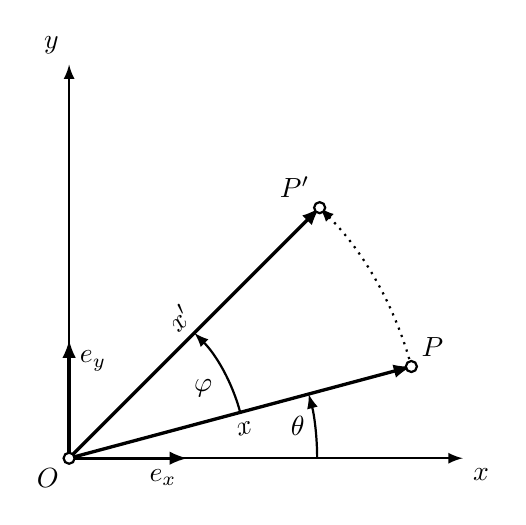
\begin{tikzpicture}
    %----------------------------------------------------------------------------------------%
    % Mathematik
    %----------------------------------------------------------------------------------------%
    \def\r{4.5};
    \def\u{30};
    \def\v{15};
    \pgfmathsetmacro\rxa{cos(\u)*\r};
    \pgfmathsetmacro\rya{sin(\u)*\r};
    \pgfmathsetmacro\rxb{cos(\v)*\rxa};
    \pgfmathsetmacro\ryb{sin(\v)*\rxa};
    %----------------------------------------------------------------------------------------%
    % Koordinaten
    %----------------------------------------------------------------------------------------%
    \coordinate (O) at (0,0);
    \coordinate (P1) at (\v:\r);
    \coordinate (P2) at (\v+\u:\r);
    %----------------------------------------------------------------------------------------%
    % Koordinatenachsen
    %----------------------------------------------------------------------------------------%
    \begin{scope}[thick,->,>=latex]
    \draw (O) -- +(5,0) node[anchor=north west] {$x$};
    \draw (O) -- +(0,5) node[anchor=south east] {$y$};
    \end{scope}
    %----------------------------------------------------------------------------------------%
    % Einheitsvektoren
    %----------------------------------------------------------------------------------------%
    \begin{scope}[very thick,->,>=latex,scale = 1.5]
    \draw (O) -- +(1,0) node[anchor = north east] {$\bvec{e_{x}}$};
    \draw (O) -- +(0,1) node[anchor = north west] {$\bvec{e_{y}}$};
    \end{scope}
    %----------------------------------------------------------------------------------------%
    % Vektoren
    %----------------------------------------------------------------------------------------%
    \begin{scope}[very thick,->,>=latex]
    \draw (O) -- (P1) node [midway, sloped, below] {$\bvec{x}$};
    \draw (O) -- (P2) node [midway, sloped, above] {$\bvec{x}^\prime$};
    \end{scope}
    %----------------------------------------------------------------------------------------%
    % Winkelbögen
    %----------------------------------------------------------------------------------------%
    \begin{scope}[thick,->,>=latex]
    \draw (P1)+(180+\v:\r/2) arc (\v:\v+\u:\r/2) node [midway, anchor = north east] {$\varphi$};
    \draw (0:\r*0.7) arc (0:\v:\r*0.7) node [midway, anchor = east] {$\theta$};
    \draw[dotted] (P1)+(180+\v:0) arc (\v:\v+\u:\r);
    \end{scope}
    %----------------------------------------------------------------------------------------%
    % Punkte
    %----------------------------------------------------------------------------------------%
    \begin{scope}[thick,draw=black,fill=white]
    \filldraw (O) circle (2pt) node[anchor=north east] {$O$};
    \filldraw (P1) circle (2pt) node[anchor=south west] {$P$};
    \filldraw (P2) circle (2pt) node[anchor=south east] {$P^\prime$};
    \end{scope}
    %----------------------------------------------------------------------------------------%
\end{tikzpicture}
        \caption{Drehung des Objekts}\label{fig:rotation_2d_a}
    \end{subfigure}
    \begin{subfigure}[b]{0.45\textwidth}
        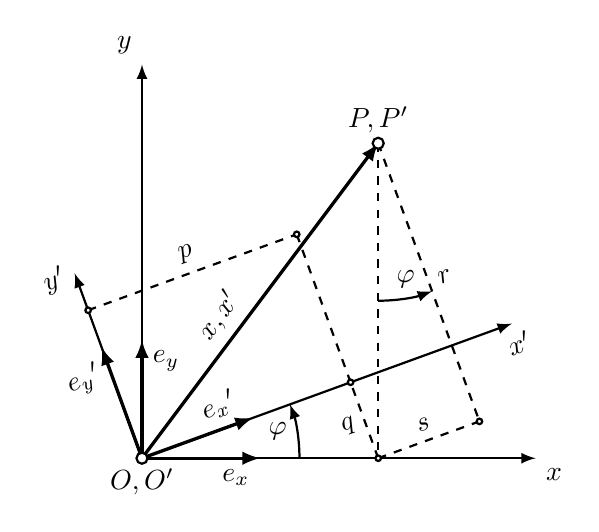
\begin{tikzpicture}
    %----------------------------------------------------------------------------------------%
    % Mathematik
    %----------------------------------------------------------------------------------------%
    \def\r{2};
    \def\u{20};
    \def\x{3};
    \def\y{4};
    \pgfmathsetmacro\xc{cos(\u)*\x};
    \pgfmathsetmacro\yc{cos(\u)*\y};
    \pgfmathsetmacro\xs{sin(\u)*\x};
    \pgfmathsetmacro\ys{sin(\u)*\y};
    %----------------------------------------------------------------------------------------%
    % Koordinaten
    %----------------------------------------------------------------------------------------%
    \coordinate (O) at (0,0);
    \coordinate (P1) at (\x,\y);
    \path (P1) -- (O-|P1) coordinate (S1);
    \path (P1) +(\u-90:\yc) coordinate (S2);
    \path (S1) +(\u+90:\xs) coordinate (S3);
    \path (S3) +(\u+90:2) coordinate (S4);
    \path (O) +(\u+90:2) coordinate (S5);
    %----------------------------------------------------------------------------------------%
    % Koordinatenachsen
    %----------------------------------------------------------------------------------------%
    \begin{scope}[thick,->,>=latex]
    \draw (O) -- +(5,0) node[anchor=north west] {$x$};
    \draw (O) -- +(0,5) node[anchor=south east] {$y$};
    \draw (O) -- +(\u:5) node[anchor=north, rotate=\u] {$x^\prime$};
    \draw (O) -- +(\u+90:2.5) node[anchor=east, rotate=\u] {$y^\prime$};
    \end{scope}
    %----------------------------------------------------------------------------------------%
    % Einheitsvektoren
    %----------------------------------------------------------------------------------------%
    \begin{scope}[very thick,->,>=latex,scale = 1.5]
    \draw (O) -- +(1,0) node[anchor = north east] {$\bvec{e_{x}}$};
    \draw (O) -- +(0,1) node[anchor = north west] {$\bvec{e_{y}}$};
    \draw (O) -- +(\u:1) node[anchor = south east,rotate=\u] {$\bvec{e_{x}}^\prime$};
    \draw (O) -- +(\u+90:1) node[anchor = north east, rotate=\u] {$\bvec{e_{y}}^\prime$};
    \end{scope}
    %----------------------------------------------------------------------------------------%
    % Vektoren
    %----------------------------------------------------------------------------------------%
    \begin{scope}[very thick,->,>=latex]
    \draw (O) -- (P1) node [midway, sloped, anchor= south east] {$\bvec{x},\bvec{x}^\prime$};
    \end{scope}
    %----------------------------------------------------------------------------------------%
    % Komponenten
    %----------------------------------------------------------------------------------------%
    \begin{scope}[thick, dashed]
    \draw (P1) -- (S1);
    \draw (P1) -- (S2) node [midway, sloped, anchor = west, rotate=90] (TextNode) {$r$};
    \draw (S1) -- (S2) node [midway, sloped, above] (TextNode) {$s$};
    \draw (S1) -- (S3) node [midway, sloped, anchor = east, rotate=90] (TextNode) {$q$};
    \draw (S5) -- (S4) node [midway, sloped, above] (TextNode) {$p$};
    \draw (S4) -- (S3);
    \end{scope}
    %----------------------------------------------------------------------------------------%
    % Punkte
    %----------------------------------------------------------------------------------------%
    \begin{scope}[thick,draw=black,fill=white]
    \filldraw (O) circle (2pt) node[anchor=north] {$O,O^\prime$};
    \filldraw (P1) circle (2pt) node[anchor=south] {$P,P^\prime$};
    \filldraw (S1) circle (1pt);
    \filldraw (S2) circle (1pt);
    \filldraw (S3) circle (1pt);
    \filldraw (S4) circle (1pt);
    \filldraw (S5) circle (1pt);
    \end{scope}
    %----------------------------------------------------------------------------------------%
    % Winkelbögen
    %----------------------------------------------------------------------------------------%
    \begin{scope}[thick,->,>=latex]
    \draw (0:\r) arc (0:\u:\r) node [midway, anchor = east] {$\varphi$};
    \draw (P1)+(0,-\r) arc (-90:\u-90:\r) node [midway, anchor = south] {$\varphi$};
    \end{scope}
    %----------------------------------------------------------------------------------------%
\end{tikzpicture}
        \caption{Drehung des Ursprungs}\label{fig:rotation_2d_b}
    \end{subfigure}
    \caption[Rotatorische Transformation in der Ebene]{Rotatorische Transformation in der Ebene, Quelle: Eigene Darstellung}\label{fig:rotation_2d}
\end{figure}
%---------------------------------------------------------------------------------------------%
% Fall B - Drehung des Ursprungs
%---------------------------------------------------------------------------------------------%
\subsubsection{Fall B - Drehung des Ursprungs}
\cref{fig:rotation_2d_b} zeigt die Drehung des Koordinatensystems $K = \{O;\bvec{x},\bvec{y}\}$ um den Winkle $\varphi$ in das neue System $K^\prime = \{O^\prime;\bvec{x}^\prime\,\bvec{y}^\prime\}$. $P,P^\prime$ wird nicht bewegt, dafür ändern sich dessen Koordinaten, ausgedrückt durch den neuen Ortsvektor $\bvec{x}^\prime$. Zur Beschreibung der Transformation von $\bvec{x}$ nach $\bvec{x}^\prime$ lassen sich \cref{eq:rotation_2d_b5,eq:rotation_2d_b6} anhand \cref{fig:rotation_2d_b} entwicklen. Für die abgebildeten Terme lässt sich schreiben:
\begin{align}
    p &= x\cos{\varphi}\label{eq:rotation_2d_b1}\\
    q &= x\sin{\varphi}\label{eq:rotation_2d_b2}\\
    r &= y\cos{\varphi}\label{eq:rotation_2d_b3}\\
    s &= y\sin{\varphi}\label{eq:rotation_2d_b4}
\end{align}
Es folgt für die Komponenten des Vektors $\bvec{x}^\prime$:
\begin{align}
    x^\prime &= p + s = x\cos{\varphi} + y\sin{\varphi}\label{eq:rotation_2d_b5}\\
    y^\prime &= r - q = y\cos{\varphi} - x\sin{\varphi}\label{eq:rotation_2d_b6}
\end{align}
Mit der Rotationsmatrix $\bvec{R}$ ergibt sich für die Transformationsgleichung in Vektorform:
\begin{gather}
    \bvec{R}=
    \begin{pmatrix}
        \cos{\varphi} & \sin{\varphi} \\
        -\sin{\varphi} & \cos{\varphi} 
    \end{pmatrix}
    \label{eq:rotation_2d_b7}
\end{gather}
\begin{equation}
    \bvec{x}^\prime = \bvec{R}\bvec{x} \label{eq:rotation_2d_b8}
\end{equation}
Bei Gegenüberstellung der Rotationsmatrizen aus \textbf{Fall A} \bref{eq:rotation_2d_a3} mit jener aus \textbf{Fall B} \bref{eq:rotation_2d_b7} zeigt sich der charakteristische Vorzeichenwechsel, wie er schon aus der Translation bekannt ist. Die Rotationsmatrizen sind orthogonal, womit allgemein gilt:
\begin{equation}
    \bvec{R}^{-1} = \bvec{R}^{T}\label{eq:rotation_2d_b9}
\end{equation}
Es kann damit erneut gezeigt werden, dass die Transformation für den \textbf{Fall A} der \glqq inversen Transformation\grqq\ von \textbf{Fall B} entspricht, und umgekehrt.
\begin{equation}
    \bvec{R}|_{Fall\,A} = \bvec{R}^{-1}|_{Fall\,B}
    \quad\Longleftrightarrow\quad
    \bvec{R}|_{Fall\,B} = \bvec{R}^{-1}|_{Fall\,A}
    \label{eq:rotation_2d_b10}
\end{equation}
%---------------------------------------------------------------------------------------------%
% Subsection: Zusammengesetzte Transformation in der Ebene
%---------------------------------------------------------------------------------------------%
\subsection{Zusammengesetzte Transformationen in der Ebene}
\label{subsec:transformation_2d}
\begin{equation}
    \bvec{R}^{-1} = \bvec{R}^{T}\label{eq:rotation_2d_b9}
\end{equation}
\begin{equation}
    \bvec{R}^{-1} = \bvec{R}^{T}\label{eq:rotation_2d_b9}
\end{equation}

%---------------------------------------------------------------------------------------------%
% Subsection: Zusammengestzte Transformation in der Ebene
%---------------------------------------------------------------------------------------------%
\subsection{Transformationen im Raum}
\label{subsec:translation_2d}

\begin{figure}[H]
    \centering
    \tdplotsetmaincoords{60}{60}

\begin{center}
\begin{tikzpicture}[scale=0.2,tdplot_main_coords]
%---------------------------------------------------------------------------------------------------%
% define coordinates
%---------------------------------------------------------------------------------------------------%
\coordinate (R) at (0,0,0);
\coordinate (P) at (15,5,25);
%---------------------------------------------------------------------------------------------------%
% input macro to replace rotationmatrix
%---------------------------------------------------------------------------------------------------%
\input{macros/rotation_xyz.tex}
%---------------------------------------------------------------------------------------------------%
% define unit-vector lengths
%---------------------------------------------------------------------------------------------------%
\def\ux{10}
\def\uy{10}
\def\uz{10}
%---------------------------------------------------------------------------------------------------%
\begin{scope}[very thick,->,>=latex]
\draw (R) -- ++(\ux,0,0) node[anchor=north]{$\bvec{x}_R$};
\draw (R) -- ++(0,\uy,0) node[anchor=south]{$\bvec{y}_R$};
\draw (R) -- ++(0,0,\uz) node[anchor=east]{$\bvec{z}_R$};
\node at (R) [anchor=north east]{$\{R\}$};
\end{scope}

\draw[very thick,->,>=spaced latex] (R) -- (P) node[midway,left]{${}^R\bvec{r}_P$};
\filldraw[thick,draw=black,fill=white] (P) circle (10pt) node[anchor=north west] {$P$};

\end{tikzpicture}
\end{center}
    \caption{Ortsvektor}\label{fig:trans3d_ortsvektor}
\end{figure}

\begin{figure}[H]
    \centering
    \tdplotsetmaincoords{60}{60}

\begin{center}
\begin{tikzpicture}[scale=0.2,tdplot_main_coords]
%---------------------------------------------------------------------------------------------------%
% define coordinates
%---------------------------------------------------------------------------------------------------%
\coordinate (R) at (0,0,0);
\coordinate (P) at (5,5,25);
\coordinate (B) at (0,25,10);
%---------------------------------------------------------------------------------------------------%
% input macro to replace rotationmatrix
%---------------------------------------------------------------------------------------------------%
\input{macros/rotation_xyz.tex}
%---------------------------------------------------------------------------------------------------%
% define unit-vector lengths
%---------------------------------------------------------------------------------------------------%
\def\ux{10}
\def\uy{10}
\def\uz{10}
%---------------------------------------------------------------------------------------------------%
\begin{scope}[very thick,->,>=latex]
\draw (R) -- ++(\ux,0,0) node[anchor=north]{$\bvec{x}_R$};
\draw (R) -- ++(0,\uy,0) node[anchor=south]{$\bvec{y}_R$};
\draw (R) -- ++(0,0,\uz) node[anchor=east]{$\bvec{z}_R$};
\end{scope}
\node at (R) [anchor=north east]{$\{R\}$};

\tdsetxyzrel
\tdplotsetrotatedcoordsorigin{(B)}
\tdplotsetrotatedcoords{10}{-25}{20}
\begin{scope}[very thick,->,>=latex,tdplot_rotated_coords]
\draw (B) -- ++(\ux,0,0) node[anchor=north]{$\bvec{x}_B$};
\draw (B) -- ++(0,\uy,0) node[anchor=south]{$\bvec{y}_B$};
\draw (B) -- ++(0,0,\uz) node[anchor=east]{$\bvec{z}_B$};
\end{scope}
\node at (B) [anchor=north west]{$\{B\}$};

\begin{scope}[very thick,->,>=spaced latex]
\draw (R) -- (P) node[midway,anchor=south east]{${}^R\bvec{r}_P$};
\draw (R) -- (B) node[midway,anchor=north west]{${}^R\bvec{r}_{O,B}$};
\draw (B) -- (P) node[midway,anchor=south west]{${}^B\bvec{r}_P$};
\end{scope}

\filldraw[thick,draw=black,fill=white] (P) circle (10pt) node[anchor=south east] {$P$};

\end{tikzpicture}
\end{center}

    \caption{Transformationsbeziheung}\label{fig:trans3d_beziehung}
\end{figure}

\begin{figure}[H]
    \centering
    \tdplotsetmaincoords{80}{30}

\begin{center}
\begin{tikzpicture}[scale=0.2,tdplot_main_coords]
%---------------------------------------------------------------------------------------------------%
% define coordinates
%---------------------------------------------------------------------------------------------------%
\coordinate (P) at (5,5,30);
\coordinate (A) at (0,0,0);
\coordinate (B) at (30,5,15);
\coordinate (C) at (50,15,30);
%---------------------------------------------------------------------------------------------------%
% input macro to replace rotationmatrix
%---------------------------------------------------------------------------------------------------%
\input{macros/rotation_xyz.tex}
%---------------------------------------------------------------------------------------------------%
% define unit-vector lengths
%---------------------------------------------------------------------------------------------------%
\def\ux{10}
\def\uy{10}
\def\uz{10}
%---------------------------------------------------------------------------------------------------%
\begin{scope}[very thick,->,>=latex]
\draw (A) -- ++(\ux,0,0) node[anchor=north]{$\bvec{x}_A$};
\draw (A) -- ++(0,\uy,0) node[anchor=south]{$\bvec{y}_A$};
\draw (A) -- ++(0,0,\uz) node[anchor=east]{$\bvec{z}_A$};
\end{scope}
\node at (A) [anchor=north]{$\{A\}$};

\tdsetxyzrel
\tdplotsetrotatedcoordsorigin{(B)}
\tdplotsetrotatedcoords{10}{0}{0}
\begin{scope}[very thick,->,>=latex,tdplot_rotated_coords]
\draw (B) -- ++(\ux,0,0) node[anchor=north]{$\bvec{x}_B$};
\draw (B) -- ++(0,\uy,0) node[anchor=south]{$\bvec{y}_B$};
\draw (B) -- ++(0,0,\uz) node[anchor=east]{$\bvec{z}_B$};
\end{scope}
\node at (B) [anchor=north west]{$\{B\}$};

\tdsetxyzrel
\tdplotsetrotatedcoordsorigin{(C)}
\tdplotsetrotatedcoords{10}{-20}{0}
\begin{scope}[very thick,->,>=latex,tdplot_rotated_coords]
\draw (C) -- ++(\ux,0,0) node[anchor=north]{$\bvec{x}_C$};
\draw (C) -- ++(0,\uy,0) node[anchor=south]{$\bvec{y}_C$};
\draw (C) -- ++(0,0,\uz) node[anchor=east]{$\bvec{z}_C$};
\end{scope}
\node at (C) [anchor=north west]{$\{C\}$};


\draw[thick,->,>=spaced latex,bend right] (A) to node[midway,anchor=north west]{${}^A_B T$} (B);
\draw[thick,->,>=spaced latex,bend right] (B) to node[midway,anchor=north west]{${}^B_C T$} (C);

\begin{scope}[very thick,->,>=spaced latex]
\draw (A) -- (P) node[midway,anchor=south east]{${}^A\bvec{r}_P$};
\draw (B) -- (P) node[midway,anchor=north east]{${}^B\bvec{r}_P$};
\draw (C) -- (P) node[midway,anchor=south west]{${}^C\bvec{r}_P$};
\end{scope}

\filldraw[thick,draw=black,fill=white] (P) circle (10pt) node[anchor=south east] {$P$};

\end{tikzpicture}
\end{center}

    \caption{Transformationsarithmetik}\label{fig:trans3d_arithmetik}
\end{figure}

\begin{figure}[H]
    \centering
    \tdplotsetmaincoords{60}{60}

\begin{center}
\begin{tikzpicture}[scale=0.2,tdplot_main_coords]
%---------------------------------------------------------------------------------------------------%
% define coordinates
%---------------------------------------------------------------------------------------------------%
\coordinate (P) at (-22,35,10);
\coordinate (A) at (0,0,0);
\coordinate (B) at (20,30,-5);
%---------------------------------------------------------------------------------------------------%
% input macro to replace rotationmatrix
%---------------------------------------------------------------------------------------------------%
\input{macros/rotation_xyz.tex}
%---------------------------------------------------------------------------------------------------%
% define unit-vector lengths
%---------------------------------------------------------------------------------------------------%
\def\ux{10}
\def\uy{10}
\def\uz{10}
%---------------------------------------------------------------------------------------------------%
\begin{scope}[very thick,->,>=latex]
\draw (A) -- ++(\ux,0,0) node[anchor=north]{$\bvec{x}_A$};
\draw (A) -- ++(0,\uy,0) node[anchor=south]{$\bvec{y}_A$};
\draw (A) -- ++(0,0,\uz) node[anchor=east]{$\bvec{z}_A$};
\end{scope}
\node at (A) [anchor=north east]{$\{A\}$};

\tdsetxyzrel
\tdplotsetrotatedcoordsorigin{(B)}
\tdplotsetrotatedcoords{0}{0}{-35}
\begin{scope}[very thick,->,>=latex,tdplot_rotated_coords]
\draw (B) -- ++(\ux,0,0) node[anchor=north]{$\bvec{x}_B$};
\draw (B) -- ++(0,\uy,0) node[anchor=south]{$\bvec{y}_B$};
\draw (B) -- ++(0,0,\uz) node[anchor=east]{$\bvec{z}_B$};
\end{scope}
\node at (B) [anchor= north west]{$\{B\}$};

\begin{scope}[very thick,->,>=spaced latex]
\draw (A) -- (P) node[midway,anchor=south east]{${}^A\bvec{r}_P$};
\draw (B) -- (P) node[midway,anchor=south west]{${}^B\bvec{r}_P$};
\draw (A) -- (B) node[midway,above,sloped]{${}^A\bvec{r}_{O,B}=-{}^B\bvec{r}_{O,A}$};
\end{scope}

\draw[thick,->,>=spaced latex] (A) to [bend right=25] node[midway,anchor=north west]{${}^A_B T$} (B);

\filldraw[thick,draw=black,fill=white] (P) circle (10pt) node[anchor=south east] {$P$};

\end{tikzpicture}
\end{center}

    \caption{Berechnung des inversen Frames}\label{fig:trans3d_inverse}
\end{figure}

\begin{figure}[H]
    \centering
    \tdplotsetmaincoords{80}{30}

\begin{center}
\begin{tikzpicture}[scale=0.2,tdplot_main_coords]
%---------------------------------------------------------------------------------------------------%
% define coordinates
%---------------------------------------------------------------------------------------------------%
\coordinate (R) at (0,0,0);
\coordinate (A0) at (10,25,5);
\coordinate (A1) at (10,25,25);
\coordinate (A2) at (10,25,45);
\coordinate (B0) at (30,50,4);
\coordinate (B1) at (30,50,24);
\coordinate (B2) at (30,50,43);

%---------------------------------------------------------------------------------------------------%
% input macro to replace rotationmatrix
%---------------------------------------------------------------------------------------------------%
\input{macros/rotation_xyz.tex}
%---------------------------------------------------------------------------------------------------%
% define unit-vector lengths
%---------------------------------------------------------------------------------------------------%
\def\ux{10}
\def\uy{10}
\def\uz{10}
%---------------------------------------------------------------------------------------------------%
\begin{scope}[very thick,->,>=latex]
\draw (R) -- ++(\ux,0,0) node[anchor=north]{$\bvec{x}_R$};
\draw (R) -- ++(0,\uy,0) node[anchor=south]{$\bvec{y}_R$};
\draw (R) -- ++(0,0,\uz) node[anchor=east]{$\bvec{z}_R$};
\end{scope}
\node at (R) [anchor=north east]{$\{R\}$};

\begin{scope}[very thick,->,>=latex]
\draw (A0) -- ++(\ux,0,0) node[anchor=north]{$\bvec{x}_{A_0}$};
\draw (A0) -- ++(0,\uy,0) node[anchor=south]{$\bvec{y}_{A_0}$};
\draw (A0) -- ++(0,0,\uz) node[anchor=east]{$\bvec{z}_{A_0}$};
\end{scope}
\node at (A0) [anchor=north east]{$\{A_0\}$};

\tdsetxyzabs
\tdplotsetrotatedcoordsorigin{(A1)}
\tdplotsetrotatedcoords{90}{0}{0}
\begin{scope}[very thick,->,>=latex,tdplot_rotated_coords]
\draw (A1) -- ++(\ux,0,0) node[anchor=north]{$\bvec{x}_{A_1}$};
\draw (A1) -- ++(0,\uy,0) node[anchor=south]{$\bvec{y}_{A_1}$};
\draw (A1) -- ++(0,0,\uz) node[anchor=east]{$\bvec{z}_{A_1}$};
\end{scope}
\node at (A1) [anchor= south east]{$\{A_1\}$};

\tdsetxyzabs
\tdplotsetrotatedcoordsorigin{(A2)}
\tdplotsetrotatedcoords{90}{0}{90}
\begin{scope}[very thick,->,>=latex,tdplot_rotated_coords]
\draw (A2) -- ++(\ux,0,0) node[anchor=south]{$\bvec{x}_{A_2}$};
\draw (A2) -- ++(0,\uy,0) node[anchor=south]{$\bvec{y}_{A_2}$};
\draw (A2) -- ++(0,0,\uz) node[anchor=north]{$\bvec{z}_{A_2}$};
\end{scope}
\node at (A2) [anchor= east]{$\{A_2\}$};

\begin{scope}[very thick,->,>=latex]
\draw (B0) -- ++(\ux,0,0) node[anchor=north]{$\bvec{x}_{B_0}$};
\draw (B0) -- ++(0,\uy,0) node[anchor=south]{$\bvec{y}_{B_0}$};
\draw (B0) -- ++(0,0,\uz) node[anchor=east]{$\bvec{z}_{B_0}$};
\end{scope}
\node at (B0) [anchor=north east]{$\{B_0\}$};

\tdsetxyzrel
\tdplotsetrotatedcoordsorigin{(A1)}
\tdplotsetrotatedcoords{90}{0}{0}
\begin{scope}[very thick,->,>=latex,tdplot_rotated_coords]
\draw (B1) -- ++(\ux,0,0) node[anchor=north]{$\bvec{x}_{B_1}$};
\draw (B1) -- ++(0,\uy,0) node[anchor=south]{$\bvec{y}_{B_1}$};
\draw (B1) -- ++(0,0,\uz) node[anchor=east]{$\bvec{z}_{B_1}$};
\end{scope}
\node at (B1) [anchor= south east]{$\{B_1\}$};

\tdsetxyzrel
\tdplotsetrotatedcoordsorigin{(A2)}
\tdplotsetrotatedcoords{90}{0}{90}
\begin{scope}[very thick,->,>=latex,tdplot_rotated_coords]
\draw (B2) -- ++(\ux,0,0) node[anchor=south]{$\bvec{x}_{B_2}$};
\draw (B2) -- ++(0,\uy,0) node[anchor=south]{$\bvec{y}_{B_2}$};
\draw (B2) -- ++(0,0,\uz) node[anchor=east]{$\bvec{z}_{B_2}$};
\end{scope}
\node at (B2) [anchor= west]{$\{B_2\}$};

\draw[thick,->,>=spaced latex] (A0) to [bend right=35] node[midway,anchor=west]{$Rot(\bvec{x}_R,90\si{\degree})$} (A1);
\draw[thick,->,>=spaced latex] (A1) to [bend right=35] node[midway,anchor=west]{$Rot(\bvec{z}_R,90\si{\degree})$} (A2);

\draw[thick,->,>=spaced latex] (B0) to [bend right=35] node[midway,anchor=west]{$Rot(\bvec{x}_{B_0},90\si{\degree})$} (B1);
\draw[thick,->,>=spaced latex] (B1) to [bend right=35] node[midway,anchor=west]{$Rot(\bvec{z}_{B_1},90\si{\degree})$} (B2);

\end{tikzpicture}
\end{center}
    \caption{Absolute und relative Transformation von Frames}\label{fig:trans3d_absrel}
\end{figure}